% Type of the document
\documentclass{beamer}

% elementary packages:
\usepackage{graphicx}
\usepackage[latin1]{inputenc}
\usepackage[T1]{fontenc}
\usepackage[english]{babel}
\usepackage{listings}
\usepackage{xcolor}
\usepackage{eso-pic}
\usepackage{mathrsfs}
\usepackage{url}
\usepackage{amssymb}
\usepackage{amsmath}
\usepackage{multirow}
\usepackage{hyperref}
\usepackage{booktabs}
\usepackage{tikz}

% additional packages
\usepackage{bbm}

% packages supplied with ise-beamer:
\usepackage{cooltooltips}
\usepackage{colordef}
\usepackage{beamerdefs}
\usepackage{lvblisting}

% Change the pictures here:
% logobig and logosmall are the internal names for the pictures: do not modify them. 
% Pictures must be supplied as JPEG, PNG or, to be preferred, PDF
\pgfdeclareimage[height=2cm]{logobig}{hulogo}
% Supply the correct logo for your class and change the file name to "logo". The logo will appear in the lower
% right corner:
\pgfdeclareimage[height=0.7cm]{logosmall}{hulogo}

% Title page outline:
% use this number to modify the scaling of the headline on title page
\renewcommand{\titlescale}{1.0}
% the title page has two columns, the following two values determine the percentage each one should get
\renewcommand{\titlescale}{1.0}
\renewcommand{\leftcol}{0.6}

% Define the title.Don't forget to insert an abbreviation instead 
% of "title for footer". It will appear in the lower left corner:
\title{Analyzing the Ringelmann Effect with the Repeated Measures ANOVA }
% Define the authors:
\authora{Nikolas H�ft\\
	Constantin Meyer-Grant\\
	Joachim Munch\\
	Quang Nguyen Duc\\
	Frederik Schreck} % a-c
\authorb{}
\authorc{}




% Define any internet addresses, if you want to display them on the title page:
\def\linka{}
\def\linkb{}
\def\linkc{}
% Define the institute:
\institute{Statistical Programming Languages\\
	Humboldt-Universit�t zu Berlin}

% Comment the following command, if you don't want, that the pdf file starts in full screen mode:
\hypersetup{pdfpagemode=FullScreen}

%Start of the document
\begin{document}

% create the title slide, layout controlled in beamerdefs.sty and the foregoing specifications
\frame[plain]{\titlepage}

% The titles of the different sections of you talk, can be included via the \section command. The title will be displayed in the upper left corner. To indicate a new section, repeat the \section command with, of course, another section title
%%%%%%%%%%%%%%%%%%%%%%%%%%%%%%%%%%%%%%%%%%%%%%%%%%%%%%%%%%%%%%%%%%%%%%%%%%%%%%%%%%%%%%%%%%%%%%%%%%%%%%%%%%%%%%%%%%%%%%%%
\section{Introduction}
%%%%%%%%%%%%%%%%%%%%%%%%%%%%%%%%%%%%%%%%%%%%%%%%%%%%%%%%%%%%%%%%%%%%%%%%%%%%%%%%%%%%%%%%%%%%%%%%%%%%%%%%%%%%%%%%%%%%%%%%

% (A numbering of the slides can be useful for corrections, especially if you are
% dealing with large tex-files)

%%%%%%%%%%%%%%%%%%%%%%%%%%%%%%%%%%%%%%%%%%%%%%%%%%%%%%%%%%%%%%%%%%%%%%%%%%%%%%%%%%%%%%%%%%%%%%%%%%%%%%%%%%%%%%%%%%%%%%%%

% No number on outline slide
\section{}
\useheadtemplate{%
    \raisebox{-0.75cm}{\parbox{\textwidth}{%
            \footnotesize{\color{isegray}%
                \insertsection\ \leavevmode\leaders\hrule height3.2pt depth-2.8pt\hfill\kern0pt\ }}}
}

%%%%%%%%%%%%%%%%%%%%%%%%%%%%%%%%%%%%%%%%%%%%%%%%%%%%%%%%%%%%%%%%%%%%%%%%%%%%%%%%%%%%%%%%%%%%%%%%%%%%%%%%%%%%%%%%%%%%%%%%

\frame[containsverbatim]{
	\frametitle{MAGA: The Package to make ANOVA great again}
	\begin{itemize}
		\item The package bundles functionalities around the grand topic of one-way repeated measures ANOVA.
		\item Some of the functionalities have not been implemented in R yet. This package aims to fill this void.
		\item Each core functionality of the package represents a quantlet.
		\item After presenting the theory and code examples from the package, we will give a short overview of the technical implementation.
	
		
		
	\end{itemize}
}
%%%%%%%%%%%%%%%%%%%%%%%%%%%%%%%%%%%%%%%%%%%%%%%%%%%%%%%%%%%%%%%%%%%%%%%%%%%%%%%%%%%%%%%%%%%%%%%%%%%%%%%%%%%%%%%%%%%%%%%%

\frame{
\frametitle{Outline}

\begin{enumerate}
\item The Ringelmann Effect
\item The Repeated Measures ANOVA
	\begin{enumerate}
	\item Based on the ANOVA Model
	\item An Advantageous Model
	\item Confidence Intervals
	\item Effect Size Measures
	\end{enumerate}
\item Sphericity
\item Orthogonal Polynomial Contrasts
\item Our Package
	\begin{enumerate}
		\item Motivation for Making a Package
		\item Tools to Create a Package in R
		\item Things to Consider
	\end{enumerate}
\end{enumerate}
}

% No number on outline slide
\useheadtemplate{%
    \raisebox{-0.75cm}{\parbox{\textwidth}{%
            \footnotesize{\color{isegray}%
                \insertsection\ \leavevmode\leaders\hrule height3.2pt depth-2.8pt\hfill\kern0pt\ \thesection-\thepage}}}}
\setcounter{section}{1}


%%%%%%%%%%%%%%%%%%%%%%%%%%%%%%%%%%%%%%%%%%%%%%%%%%%%%%%%%%%%%%%%%%%%%%%%%%%%%%%%%%%%%%%%%%%%%%%%%%%%%%%%%%%%%%%%%%%%%%%%
\frame[containsverbatim]{
	\frametitle{The Ringelmann Effect}
	\begin{itemize}
	\item Maximilian Ringelmann (1861-1931):
	 \begin{itemize}
	 \item French professor of agricultural engineering
	 \end{itemize}
	\item Findings:
		\begin{itemize}
			\item Work performance depends on group size
			\item Decreasing individual performance with increasing group size 
			\item Example: Pulling weights in differently sized groups
		\end{itemize}
	\end{itemize}
}

%%%%%%%%%%%%%%%%%%%%%%%%%%%%%%%%%%%%%%%%%%%%%%%%%%%%%%%%%%%%%%%%%%%%%%%%%%%%%%%%%%%%%%%%%%%%%%%%%%%%%%%%%%%%%%%%%%%%%%%%


\frame[containsverbatim]{
	\frametitle{The Ringelmann Effect}
	\begin{itemize}
	\item The Ringelmann Effect can be investigated with an experimental design
	\begin{itemize}
	\item Dependent Variable: Individual performance
	\item Independent Variable / Factor: Group size 
	\item Realization of different factor levels
	\end{itemize}
	\item For our purpose: Data simulation
	\end{itemize}
}
%%%%%%%%%%%%%%%%%%%%%%%%%%%%%%%%%%%%%%%%%%%%%%%%%%%%%%%%%%%%%%%%%%%%%%%%%%%%%%%%%%%%%%%%%%%%%%%%%%%%%%%%%%%%%%%%%%%%%%%%

\frame[containsverbatim]{
	\frametitle{Quantlet 1: Data Simulation}
	
\begin{itemize}
		\item Simulation function:
	\end{itemize}
	\begin{lstlisting}
rma_data = sim_rma_data(n = 30, k = 5, means = 
	means, poly_order = NULL, noise_sd = c(155, 65, 
	75, 15, 40), between_subject_sd = 60, NAs = 2)
	\end{lstlisting}
	\begin{itemize}
		\item Simulate deviation between subjects:
	\end{itemize}
\begin{lstlisting}
mean_deviation = rnorm(n, mean = 0, 
	sd = between_subject_sd)
ow_rma_data[, 2:(k + 1)] = ow_rma_data[, 2:(k + 1)] 
	+ mean_deviation
	\end{lstlisting}
\quantnet sim\_rma\_data

}	
	
	
%%%%%%%%%%%%%%%%%%%%%%%%%%%%%%%%%%%%%%%%%%%%%%%%%%%%%%%%%%%%%%%%%%%%%%%%%%%%%%%%%%%%%%%%%%%%%%%%%%%%%%%%%%%%%%%%%%%%%%%%

\frame[containsverbatim]{
	\frametitle{Quantlet 1: Data Simulation}	
	
	\begin{itemize}
			\item Simulate noise:
		\end{itemize}
		\begin{lstlisting}
noise = matrix(NA, nrow = n, ncol = k)
	for (i in 1:k) {noise[, i] = rnorm(n, 
	mean = 0, sd = noise_sd[i])}
ow_rma_data[, 2:(k + 1)] = ow_rma_data[, 2:(k + 1)] 
	+ noise
		\end{lstlisting}
\quantnet sim\_rma\_data
	
}	
%%%%%%%%%%%%%%%%%%%%%%%%%%%%%%%%%%%%%%%%%%%%%%%%%%%%%%%%%%%%%%%%%%%%%%%%%%%%%%%%%%%%%%%%%%%%%%%%%%%%%%%%%%%%%%%%%%%%%%%%

	\frame[containsverbatim]{
		\frametitle{The Ringelmann Effect} 
		\begin{figure}[htb]
		\begin{center}
		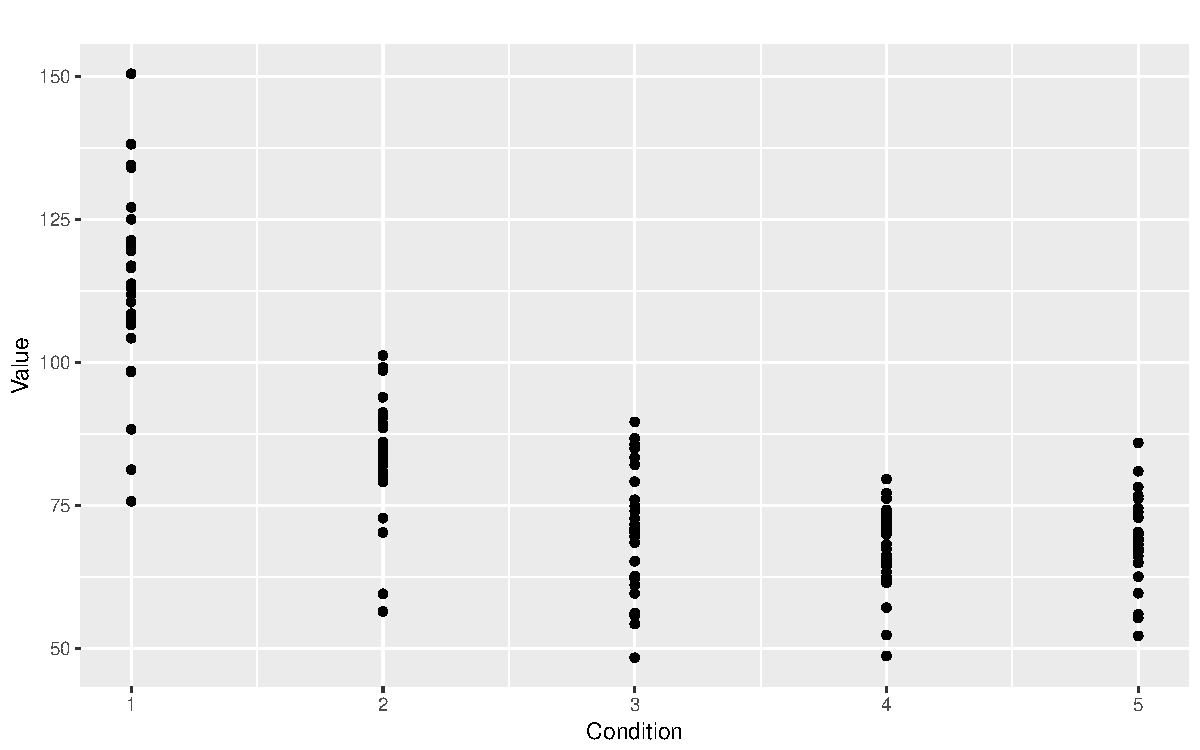
\includegraphics[scale=0.35]{dataplot.pdf}
		\caption{Simulated data.}
		\end{center}
		\end{figure}
		\quantnet sim\_rma\_data
	}

%%%%%%%%%%%%%%%%%%%%%%%%%%%%%%%%%%%%%%%%%%%%%%%%%%%%%%%%%%%%%%%%%%%%%%%%%%%%%%%%%%%%%%%%%%%%%%%%%%%%%%%%%%%%%%%%%%%%%%%%
\frame[containsverbatim]{
	\frametitle{The Repeated Measures ANOVA: Based on the ANOVA Model} 
	\begin{itemize}
	\item ANOVA: Analysis of Variance
	\item Comparison of the \textit{k} factor level means
	\item Hypotheses:
		\begin{eqnarray*}
		H_{0}: {\mu_{1}} = {\mu_{2}} = ... = {\mu_{k}} \\
		H_{1}: \exists i \not= j: {\mu_{i}} \not= {\mu_{j}} 
		\end{eqnarray*} 
		\\
	\item Test is accomplished by decomposition of variance components

	\item For dependent data: Repeated Measures ANOVA 
	\end{itemize}
}


%%%%%%%%%%%%%%%%%%%%%%%%%%%%%%%%%%%%%%%%%%%%%%%%%%%%%%%%%%%%%%%%%%%%%%%%%%%%%%%%%%%%%%%%%%%%%%%%%%%%%%%%%%%%%%%%%%%%%%%%

	\frame[containsverbatim]{
		\frametitle{The Repeated Measures ANOVA}

\begin{table}[ht]
\centering
\begin{tabular}{rrrrrr}
  \hline
 Subject & Factor.1 & Factor.2 & Factor.3 & Factor.4 & Factor.5 \\ 
  \hline
	1 & 218.25 & 147.13 & 69.18 & 74.96 & 80.11 \\ 
  2 & 173.77 & 119.62 & 114.15 & 94.04 & 87.57 \\ 
  3 & 177.49 & 116.17 & 97.97 & 72.91 & 69.28 \\ 
  4 & 126.58 & 110.36 & 123.45 & 90.82 & 75.07 \\ 
  5 & 146.61 & 108.26 & 86.91 & 76.62 & 61.94 \\ 
  6 & 167.03 & 95.48 & 72.13 & 93.29 & 102.31 \\ 
   \hline
	\end{tabular}
\caption{Our simulated data consists of dependent data.}
\end{table}
\quantnet sim\_rma\_data
		
		
	  }
	  	
%%%%%%%%%%%%%%%%%%%%%%%%%%%%%%%%%%%%%%%%%%%%%%%%%%%%%%%%%%%%%%%%%%%%%%%%%%%%%%%%%%%%%%%%%%%%%%%%%%%%%%%%%%%%%%%%%%%%%%%%

\frame[containsverbatim]{
	\frametitle{Quantlet 2: Repeated Measures ANOVA}

\begin{itemize}
	\item Repeated Measures ANOVA function: 	\quantnet rma
\end{itemize}
\begin{lstlisting}
rma(rma_data, id = 1)

\end{lstlisting}

\begin{itemize}
	\item Define basic components:
\end{itemize}

\begin{lstlisting}
grand_mean = mean(dependent_variable)
baseline_components = matrix(grand_mean, nrow = n, 
	ncol = k)
conditional_means = colMeans(dependent_variable)
factor_level_components = matrix(conditional_means -
	grand_mean, nrow = n, ncol = k, byrow = TRUE)
subject_means = rowMeans(dependent_variable)
subject_components = matrix(subject_means - 
	grand_mean, nrow = n, ncol = k)
 \end{lstlisting}   


}
%%%%%%%%%%%%%%%%%%%%%%%%%%%%%%%%%%%%%%%%%%%%%%%%%%%%%%%%%%%%%%%%%%%%%%%%%%%%%%%%%%%%%%%%%%%%%%%%%%%%%%%%%%%%%%%%%%%%%%%%

\frame[containsverbatim]{
	\frametitle{Quantlet 2: Repeated Measures ANOVA}
	
\begin{itemize}
	\item Define basic components:
\end{itemize}
\begin{lstlisting}
error_components = dependent_variable - 
	baseline_components - factor_level_components - 
	subject_components
\end{lstlisting}
	\quantnet rma
}

%%%%%%%%%%%%%%%%%%%%%%%%%%%%%%%%%%%%%%%%%%%%%%%%%%%%%%%%%%%%%%%%%%%%%%%%%%%%%%%%%%%%%%%%%%%%%%%%%%%%%%%%%%%%%%%%%%%%%%%%


\frame[containsverbatim]{
	\frametitle{The Repeated Measures ANOVA}
	
	\begin{table}[ht]
\centering
\resizebox{\textwidth}{!}{\begin{tabular}{rlrrrrr}
  \hline
 & Source & Sum of squares & Degrees of freedom & Mean squares & F-value & p-value \\ 
  \hline
1 & Baseline & 1769610.20 & 1.00 & 1769610.20 & 1430.36 & <0.001 \\ 
  2 & Factor & 174706.07 & 4.00 & 43676.52 & 142.23 & <0.001 \\ 
  3 & Subject & 33403.82 & 27.00 & 1237.18 &  &  \\ 
  4 & Error & 33166.05 & 108.00 & 307.09 &  &  \\ 
  5 & Total & 2010886.14 & 140.00 &  &  &  \\ 
  6 & Corrected total & 241275.94 & 139.00 & 1735.80 &  &  \\ 
   \hline
\end{tabular}}
\caption{ANOVA-table for our Repeated Measures ANOVA.}
\end{table}
	\quantnet rma

}

%%%%%%%%%%%%%%%%%%%%%%%%%%%%%%%%%%%%%%%%%%%%%%%%%%%%%%%%%%%%%%%%%%%%%%%%%%%%%%%%%%%%%%%%%%%%%%%%%%%%%%%%%%%%%%%%%%%%%%%%

\frame[containsverbatim]{
	\frametitle{The Repeated Measures ANOVA: An Advantageous Model}
		\begin{itemize}
		\item Problem of ANOVA: In case of large variance between different subjects\\
		$\Rightarrow$ High error variance
		$\Rightarrow$ Loss of power in F-Test
		\item Repeated Measures ANOVA considers the between subject variance separately\\
		$\Rightarrow$ Relatively low error variance
		$\Rightarrow$ Gain of power in F-Test 
		\end{itemize}
}

%%%%%%%%%%%%%%%%%%%%%%%%%%%%%%%%%%%%%%%%%%%%%%%%%%%%%%%%%%%%%%%%%%%%%%%%%%%%%%%%%%%%%%%%%%%%%%%%%%%%%%%%%%%%%%%%%%%%%%%%

\frame[containsverbatim]{
	\frametitle{Quantlet 3: ANOVA and SSE Reduction}
\begin{itemize}
	\item Reduction of sum of squares error function:
\end{itemize}
\begin{lstlisting}
rma_sse_reduct(rma_data, id = 1, 
	plot_type = "pie", return_anova_table = FALSE)

\end{lstlisting}


\begin{itemize}
	\item ANOVA function:
\end{itemize}
\begin{lstlisting}
ow_a(rma_data, id)

\end{lstlisting}
\quantnet rma\_sse\_reduct
}

%%%%%%%%%%%%%%%%%%%%%%%%%%%%%%%%%%%%%%%%%%%%%%%%%%%%%%%%%%%%%%%%%%%%%%%%%%%%%%%%%%%%%%%%%%%%%%%%%%%%%%%%%%%%%%%%%%%%%%%%

\frame[containsverbatim]{
	\frametitle{Quantlet 3: ANOVA and SSE Reduction}

\begin{itemize}
  \item ANOVA-tables of Repeated Measures ANOVA and ANOVA
\end{itemize}
\begin{lstlisting}
ow_a_results = ow_a(rma_data, id)[[1]]
rma_results = rma(rma_data, id)[[1]]
    
sse_anova = ow_a_results[3, 2]
ss_subject_anova = 0

sse_rma = rma_results[4, 2]
ss_subject_rma = rma_results[3, 2]
\end{lstlisting}
\quantnet rma\_sse\_reduct
}
%%%%%%%%%%%%%%%%%%%%%%%%%%%%%%%%%%%%%%%%%%%%%%%%%%%%%%%%%%%%%%%%%%%%%%%%%%%%%%%%%%%%%%%%%%%%%%%%%%%%%%%%%%%%%%%%%%%%%%%%

	\frame[containsverbatim]{
		\frametitle{The Repeated Measures ANOVA: An Advantageous Model} 
		\begin{figure}[htb]
		\begin{center}
		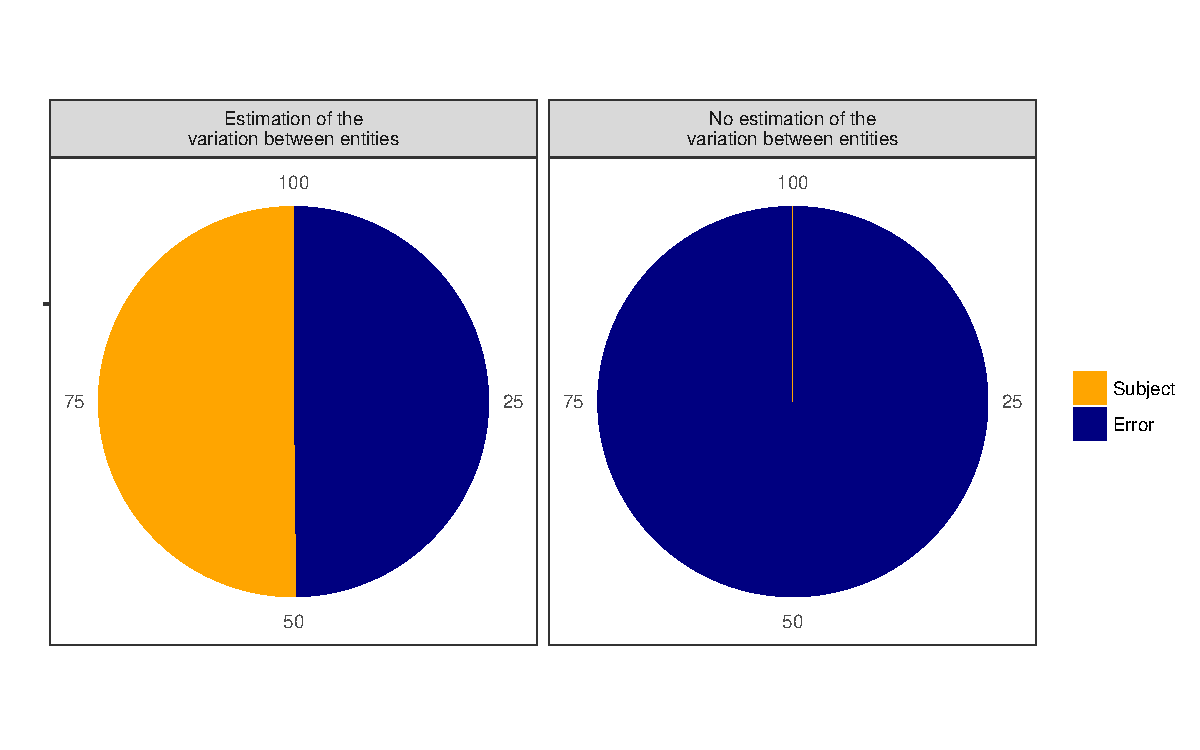
\includegraphics[scale=0.30]{sse_reduct.pdf}
		\caption{Pie chart on the reduction of sum of squares (SSE) in percentages.}
		\end{center}
		\end{figure}
		\quantnet rma\_sse\_reduct
	}
	



%%%%%%%%%%%%%%%%%%%%%%%%%%%%%%%%%%%%%%%%%%%%%%%%%%%%%%%%%%%%%%%%%%%%%%%%%%%%%%%%%%%%%%%%%%%%%%%%%%%%%%%%%%%%%%%%%%%%%%%%

\frame[containsverbatim]{
	\frametitle{The Repeated Measures ANOVA: Confidence Intervals}
	
	\begin{itemize}
	\item The computation of the confidence intervals has to be adjusted in the Repeated Measures ANOVA \quantnet rma\_ci
	\end{itemize}
	
\begin{figure}[htb]
\begin{center}
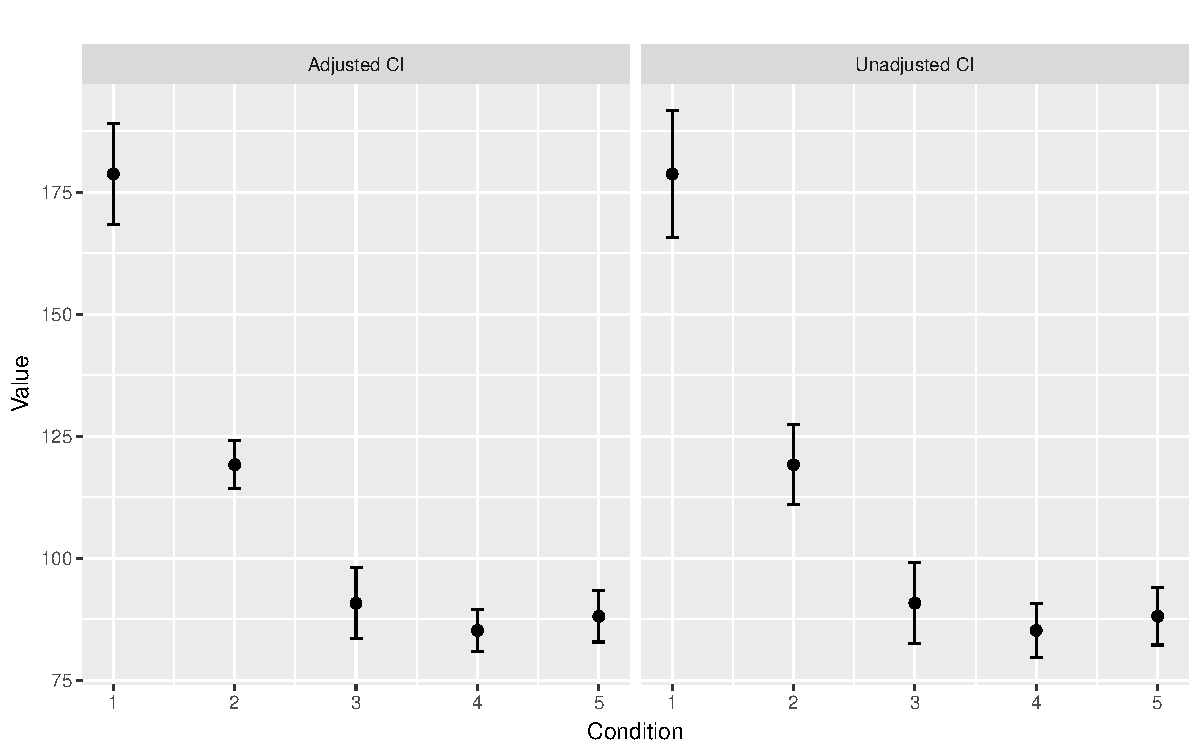
\includegraphics[scale=0.29]{CIs.pdf}
\caption{Unadjusted and adjusted confidence intervals.}
\end{center}
\end{figure}
		
}

%%%%%%%%%%%%%%%%%%%%%%%%%%%%%%%%%%%%%%%%%%%%%%%%%%%%%%%%%%%%%%%%%%%%%%%%%%%%%%%%%%%%%%%%%%%%%%%%%%%%%%%%%%%%%%%%%%%%%%%%

\frame[containsverbatim]{
	\frametitle{Quantlet 4: Confidence Intervals}

\begin{itemize}
	\item Confidence interval function:
	\end{itemize}	
\begin{lstlisting}
rma_ci(rma_data, C_level = 0.95, id = 1, print_plot = TRUE)

\end{lstlisting}


\begin{itemize}
	\item Computation of adjusted standard errors:
	\end{itemize}
\begin{lstlisting}
cf = sqrt(k/(k - 1))

AdjVal = data.frame(Adj = (cf * ((rma_data_long$value - EEmlong$Em + Gm) - MeFlmlong$Flm)) + MeFlmlong$Flm)
\end{lstlisting}  
\quantnet rma\_ci

}

	
%%%%%%%%%%%%%%%%%%%%%%%%%%%%%%%%%%%%%%%%%%%%%%%%%%%%%%%%%%%%%%%%%%%%%%%%%%%%%%%%%%%%%%%%%%%%%%%%%%%%%%%%%%%%%%%%%%%%%%%%

\frame[containsverbatim]{
	\frametitle{The Repeated Measures ANOVA: Effect Size Measures}
	\begin{itemize}
	\item Two measures of effect size: 
		\begin{itemize}
		\item $\eta^2$
		\item $\eta_{p}^2$
		\end{itemize}
	\end{itemize}
	
		\begin{table}[ht]
\centering
\begin{tabular}{rlrr}
  \hline
 & Source & eta squared & partial eta squared \\ 
  \hline
1 & Factor & 0.72 & 0.84 \\ 
   \hline
\end{tabular}
\caption{Effect size measures for our simulated data.}
\end{table}

\quantnet rma\_effect\_size
}

%%%%%%%%%%%%%%%%%%%%%%%%%%%%%%%%%%%%%%%%%%%%%%%%%%%%%%%%%%%%%%%%%%%%%%%%%%%%%%%%%%%%%%%%%%%%%%%%%%%%%%%%%%%%%%%%%%%%%%%%

\frame[containsverbatim]{
	\frametitle{Quantlet 5: Effect Size Measures}
	
\begin{itemize}
	\item Effect size measures function:
\end{itemize}

\begin{lstlisting}
rma_eta(rma_data, id = 1, append = FALSE)

\end{lstlisting}

\begin{itemize}
	\item Computation of $\eta^2$ and $\eta_{p}^2$:
\end{itemize}

\begin{lstlisting}
eta_sq = SS_Factor/SS_K_Total
    
eta_partial = SS_Factor/(SS_Factor + SS_Error)
\end{lstlisting}

\quantnet rma\_effect\_size
}

%%%%%%%%%%%%%%%%%%%%%%%%%%%%%%%%%%%%%%%%%%%%%%%%%%%%%%%%%%%%%%%%%%%%%%%%%%%%%%%%%%%%%%%%%%%%%%%%%%%%%%%%%%%%%%%%%%%%%%%%

\frame[containsverbatim]{
	\frametitle{Sphericity}
	\begin{itemize}
	\item An important requirement: The variance of differences are equal for each pair of factor levels
	\item Test for sphericity: Mauchly test
	\item Measurement of sphericity $(\epsilon \in [0, 1])$: 
		\begin{itemize}
			\item Greenhouse \& Geisser: $\epsilon_{GG}$
			\item Box: $\epsilon_{B}$
			\item Huynh \& Feldt: $\epsilon_{HF}$
		\end{itemize}
	\item These can be used to correct the degrees of freedom and therefore adjust the p-values if sphericity is violated
	\end{itemize}
}


%%%%%%%%%%%%%%%%%%%%%%%%%%%%%%%%%%%%%%%%%%%%%%%%%%%%%%%%%%%%%%%%%%%%%%%%%%%%%%%%%%%%%%%%%%%%%%%%%%%%%%%%%%%%%%%%%%%%%%%%

\frame[containsverbatim]{
	\frametitle{Quantlet 6: Test and Adjustment for Sphericity}
	
	\begin{itemize}
		\item Sphericity function:
	\end{itemize}
\begin{lstlisting}
rma_spheri(rma_data, id = 1, append = TRUE)

\end{lstlisting}

	\begin{table}[ht]
		\centering
		\begin{tabular}{rlrrrr}
			\hline
			& Source & Mauchly's W & Chi square & df & p \\ 
			\hline
			1 & Factor & 0.20 & 41.48 & 9.00 & 0.00 \\ 
			\hline
		\end{tabular}
		\caption{Result of the Mauchly test.}
	\end{table}
\quantnet rm\_spheri
}

%%%%%%%%%%%%%%%%%%%%%%%%%%%%%%%%%%%%%%%%%%%%%%%%%%%%%%%%%%%%%%%%%%%%%%%%%%%%%%%%%%%%%%%%%%%%%%%%%%%%%%%%%%%%%%%%%%%%%%%%

\frame[containsverbatim]{
	\frametitle{Sphericity}
	
\begin{table}[ht]
\centering
\begin{tabular}{rlrrr}
  \hline
 & Source & G. - G. & Box  & Huynh-Feldt  \\ 
  \hline
1 & Epsilon & 0.25 & 0.55 & 0.60 \\ 
  2 & Adj. p-Value & 0.05 & <0.001 & <0.001 \\ 
   \hline
\end{tabular}
\caption{Adjusted p-values.}
\end{table}
\quantnet rma\_spheri	
}
%%%%%%%%%%%%%%%%%%%%%%%%%%%%%%%%%%%%%%%%%%%%%%%%%%%%%%%%%%%%%%%%%%%%%%%%%%%%%%%%%%%%%%%%%%%%%%%%%%%%%%%%%%%%%%%%%%%%%%%%

\frame[containsverbatim]{
	\frametitle{Quantlet 6: Test and Adjustment for Sphericity}
	

\begin{itemize}
	\item Choose recommended adjustment: \quantnet rma\_spheri
\end{itemize}

\begin{lstlisting}  
if (p_w < 0.05) {
if (p_factor_lb < 0.05) {
 anova_table[, "Recommended Lower-Bound corrected p-Value (Greenhouse & Geisser, 1959))"] = c(NA, p_factor_lb, NA, NA, NA, NA)} 
 else {if (epsilon_gg < 0.75) {anova_table[, "Recommended Box corrected p-Value (Geisser & Greenhouse, 1958)"] = c(NA, p_factor_gg, NA, NA, NA, NA)} 
 else {anova_table[, "Recommended Huynh-Feldt corrected p-Value (Huynh & Feldt, 1976)"] = c(NA, p_factor_hf, NA, NA, NA, NA)}}}
  \end{lstlisting}

}

%%%%%%%%%%%%%%%%%%%%%%%%%%%%%%%%%%%%%%%%%%%%%%%%%%%%%%%%%%%%%%%%%%%%%%%%%%%%%%%%%%%%%%%%%%%%%%%%%%%%%%%%%%%%%%%%%%%%%%%%

\frame[containsverbatim]{
	\frametitle{Orthogonal Polynomial Contrasts}
	\begin{itemize}
		\item Further analysis of factor effect
		\item Requirement: Level of measurement at least interval
		\item Factor effect can be decomposed into polynomial trend components
		\item Polynomial trend components can be tested by polynomial contrasts
		\item If there shall be no redundant information in each trend component, the contrasts have to be orthogonal
		\begin{itemize}
			\item Maximum of orthogonal contrasts: $k-1$
		\end{itemize}
	\end{itemize}
}

%%%%%%%%%%%%%%%%%%%%%%%%%%%%%%%%%%%%%%%%%%%%%%%%%%%%%%%%%%%%%%%%%%%%%%%%%%%%%%%%%%%%%%%%%%%%%%%%%%%%%%%%%%%%%%%%%%%%%%%%

\frame[containsverbatim]{
	\frametitle{Quantlet 7: Orthogonal Polynomial Contrasts}
	
	\begin{itemize}
		\item Contrast function:
	\end{itemize}
\begin{lstlisting}
rma_opc(rma_data, id = 1, maxpoly = NA, print_plot = TRUE)

\end{lstlisting}


\begin{table}[ht]
	\centering
	\begin{tabular}{rlrrrrrrr}
		\hline
		Source & SS & Contribution & t & p \\ 
		\hline
		 .L & 32414.14 & 0.74 &  -15.67 & 0.00 \\ 
		 .Q & 10898.57 & 0.25 &  10.68 & 0.00 \\ 
		 .C & 360.39 & 0.01 & -3.40 & 0.00 \\ 
		 \verb|^|4 & 3.42 & 27.00 & -0.27 & 0.40 \\ 
		\hline
	\end{tabular}
\end{table}

\quantnet rma\_opc
}


%%%%%%%%%%%%%%%%%%%%%%%%%%%%%%%%%%%%%%%%%%%%%%%%%%%%%%%%%%%%


\frame[containsverbatim]{
	\frametitle{Plotting the Orthogonal Polynomial Curves} 
	\begin{lstlisting}
poly_plot = ggplot(data = rma_data_long, aes(x = condition, y = value)) + geom_point() + labs(col = "Order of \npolynomial", x = "Condition", y = "Value", title = "Orthogonal polynomial contrasts") + 
geom_path(data = poly_curve_data, aes(x, y, color = var), lwd = 1.2) + scale_color_discrete(labels = as.character(1:(k - 1)))	
	
	\end{lstlisting}
\quantnet rma\_opc
	
}

%%%%%%%%%%%%%%%%%%%%%%%%%%%%%%%%%%%%%%%%%%%%%%%%%%%%%%%%%%%%%%%%%%%%%%%%%%%%%%%%%%%%%%%%%%%%%%%%%%%%%%%%%%%%%%%%%%%%%%%%

\frame[containsverbatim]{
	\frametitle{Orthogonal Polynomial Contrasts} 
	\begin{figure}[htb]
		\begin{center}
			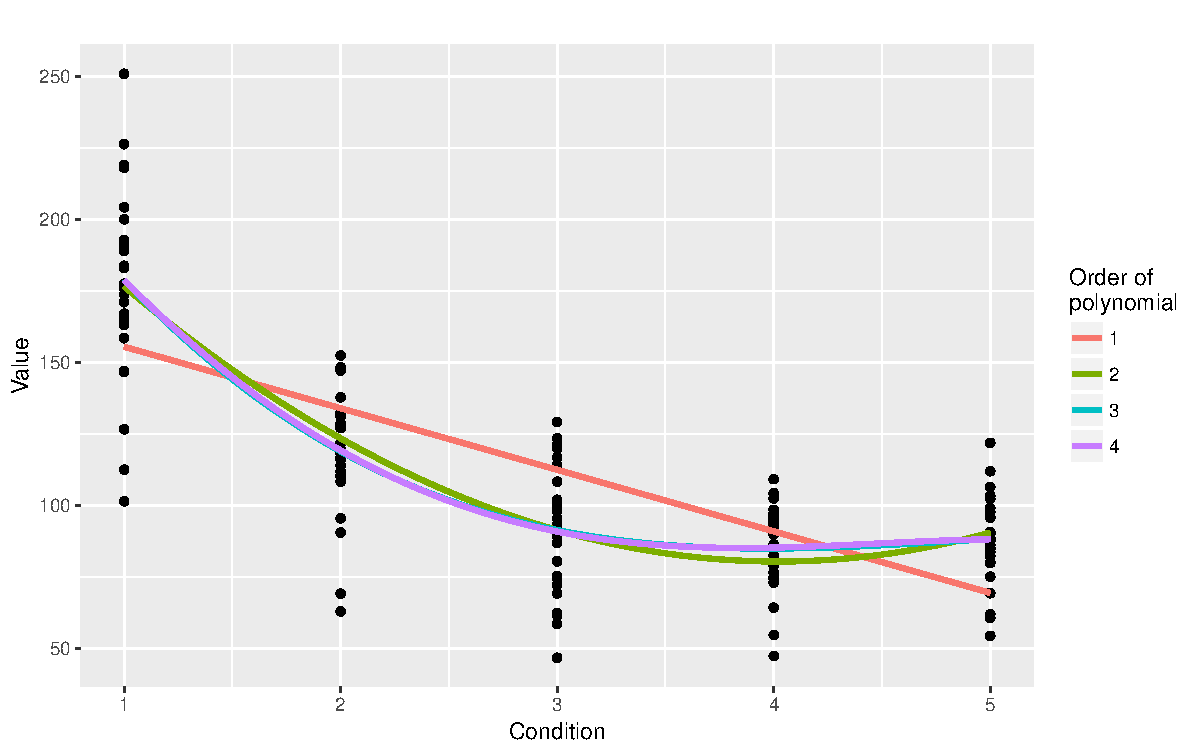
\includegraphics[scale=0.32]{opc.pdf}
			\caption{Orthogonal polynomial contrasts.}
		\end{center}
	\end{figure}
	\quantnet rma\_opc
}



%%%%%%%%%%%%%%%%%%%%%%%%%%%%%%%%%%%%%%%%%%%%%%%%%%%%%%%%%%%%


\frame[containsverbatim]{
\frametitle{Our Package: Motivation for Making a Package}

\begin{itemize}
\item A package bundles together code, data, documentation, and tests
\item Makes it easy to share and publish code with others (CRAN, Github via Devtools)
\item Loads all relevant functions into the namespace
\item Automatically checks and installs dependency if necessary
\item Packages allow to document functions, so that they easily be used by others (help function, argument list, etc.)
\end{itemize}
}

%%%%%%%%%%%%%%%%%%%%%%%%%%%%%%%%%%%%%%%%%%%%%%%%%%%%%%%%%%%%%%%%%%%%%%%%%%%%%%%%%%%%%%%%%%%%%%%%%%%%%%%%%%%%%%%%%%%%%%%%
\frame[containsverbatim]{
	\frametitle{Our Package: Tools to Create a Package\\ in R}
	
	\begin{itemize}
		\item roxygen2
		\begin{itemize}
			\item Enables documentation to be written directly into the R script
		\end{itemize}
		\item devtools
		\begin{itemize}
			\item Load packages still under development e.g. from Github
		\end{itemize}
		\item Github
		\begin{itemize}
			\item A package can be handled like a repository, which enables colloboration
		\end{itemize}
		\item RStudio
		\begin{itemize}
			\item Provides many helpful functionalities for creating a package (create, build, check)
		\end{itemize}
	\end{itemize}
}

%%%%%%%%%%%%%%%%%%%%%%%%%%%%%%%%%%%%%%%%%%%%%%%%%%%%%%%%%%%%%%%%%%%%%%%%%%%%%%%%%%%%%%%%%%%%%%%%%%%%%%%%%%%%%%%%%%%%%%%%


\frame[containsverbatim]{
	\frametitle{Create a Package in R-Studio} 
	\begin{figure}[htb]
		\begin{center}
			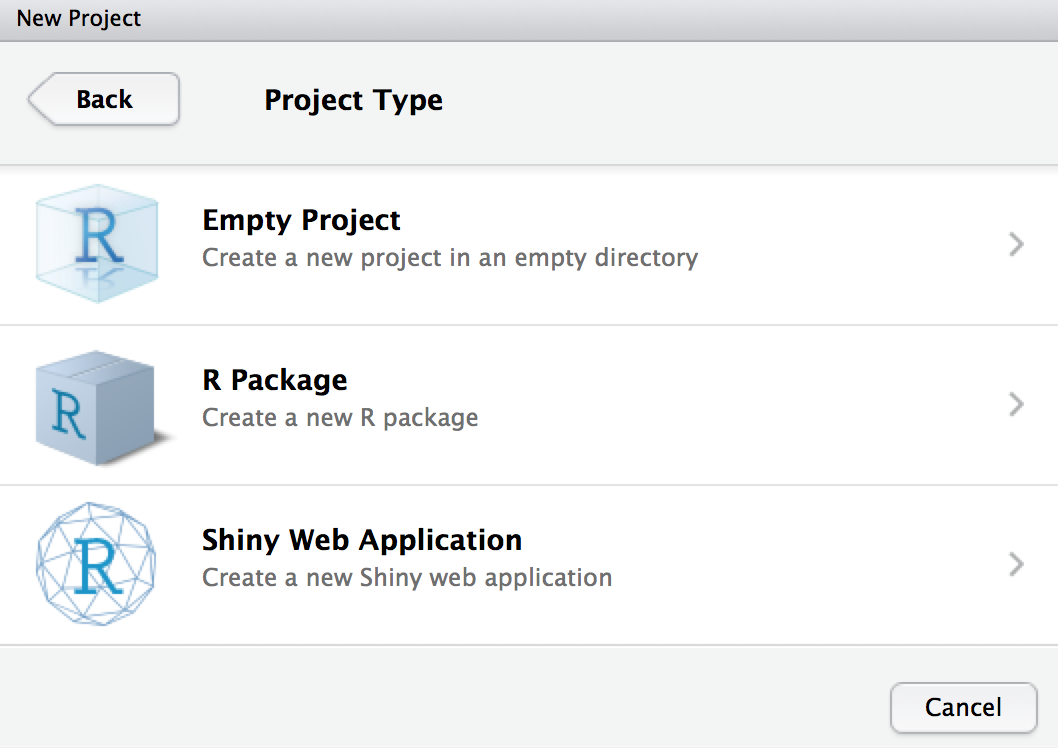
\includegraphics[scale=0.35]{create_package.png}
			\caption{Select R-Package to directly create a Package}
		\end{center}
	\end{figure}
}


%%%%%%%%%%%%%%%%%%%%%%%%%%%%%%%%%%%%%%%%%%%%%%%%%%%%%%%%%%%%%%%%%%%%%%%%%%%%%%%%%%%%%%%%%%%%%%%%%%%%%%%%%%%%%%%%%%%%%%%%

\frame[containsverbatim]{
	\frametitle{Helpfiles with roxygen2} 
	\begin{figure}[htb]
		\begin{center}
			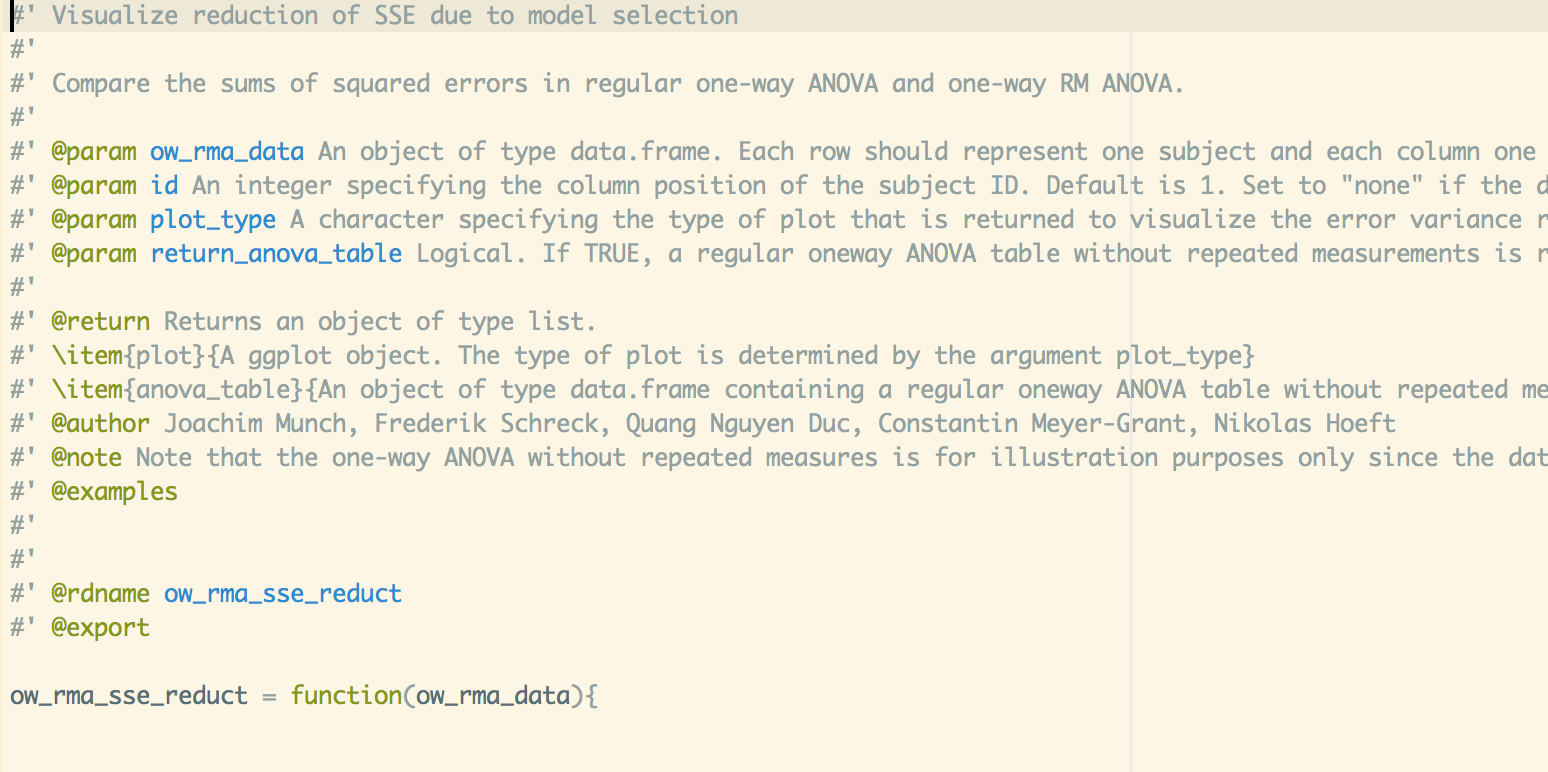
\includegraphics[scale=0.35]{roxygen_code.png}
			
		\end{center}
	\end{figure}
}


%%%%%%%%%%%%%%%%%%%%%%%%%%%%%%%%%%%%%%%%%%%%%%%%%%%%%%%%%%%%%%%%%%%%%%%%%%%%%%%%%%%%%%%%%%%%%%%%%%%%%%%%%%%%%%%%%%%%%%%%

\frame[containsverbatim]{
	\frametitle{Helpfiles with roxygen2} 
	\begin{figure}[htb]
		\begin{center}
			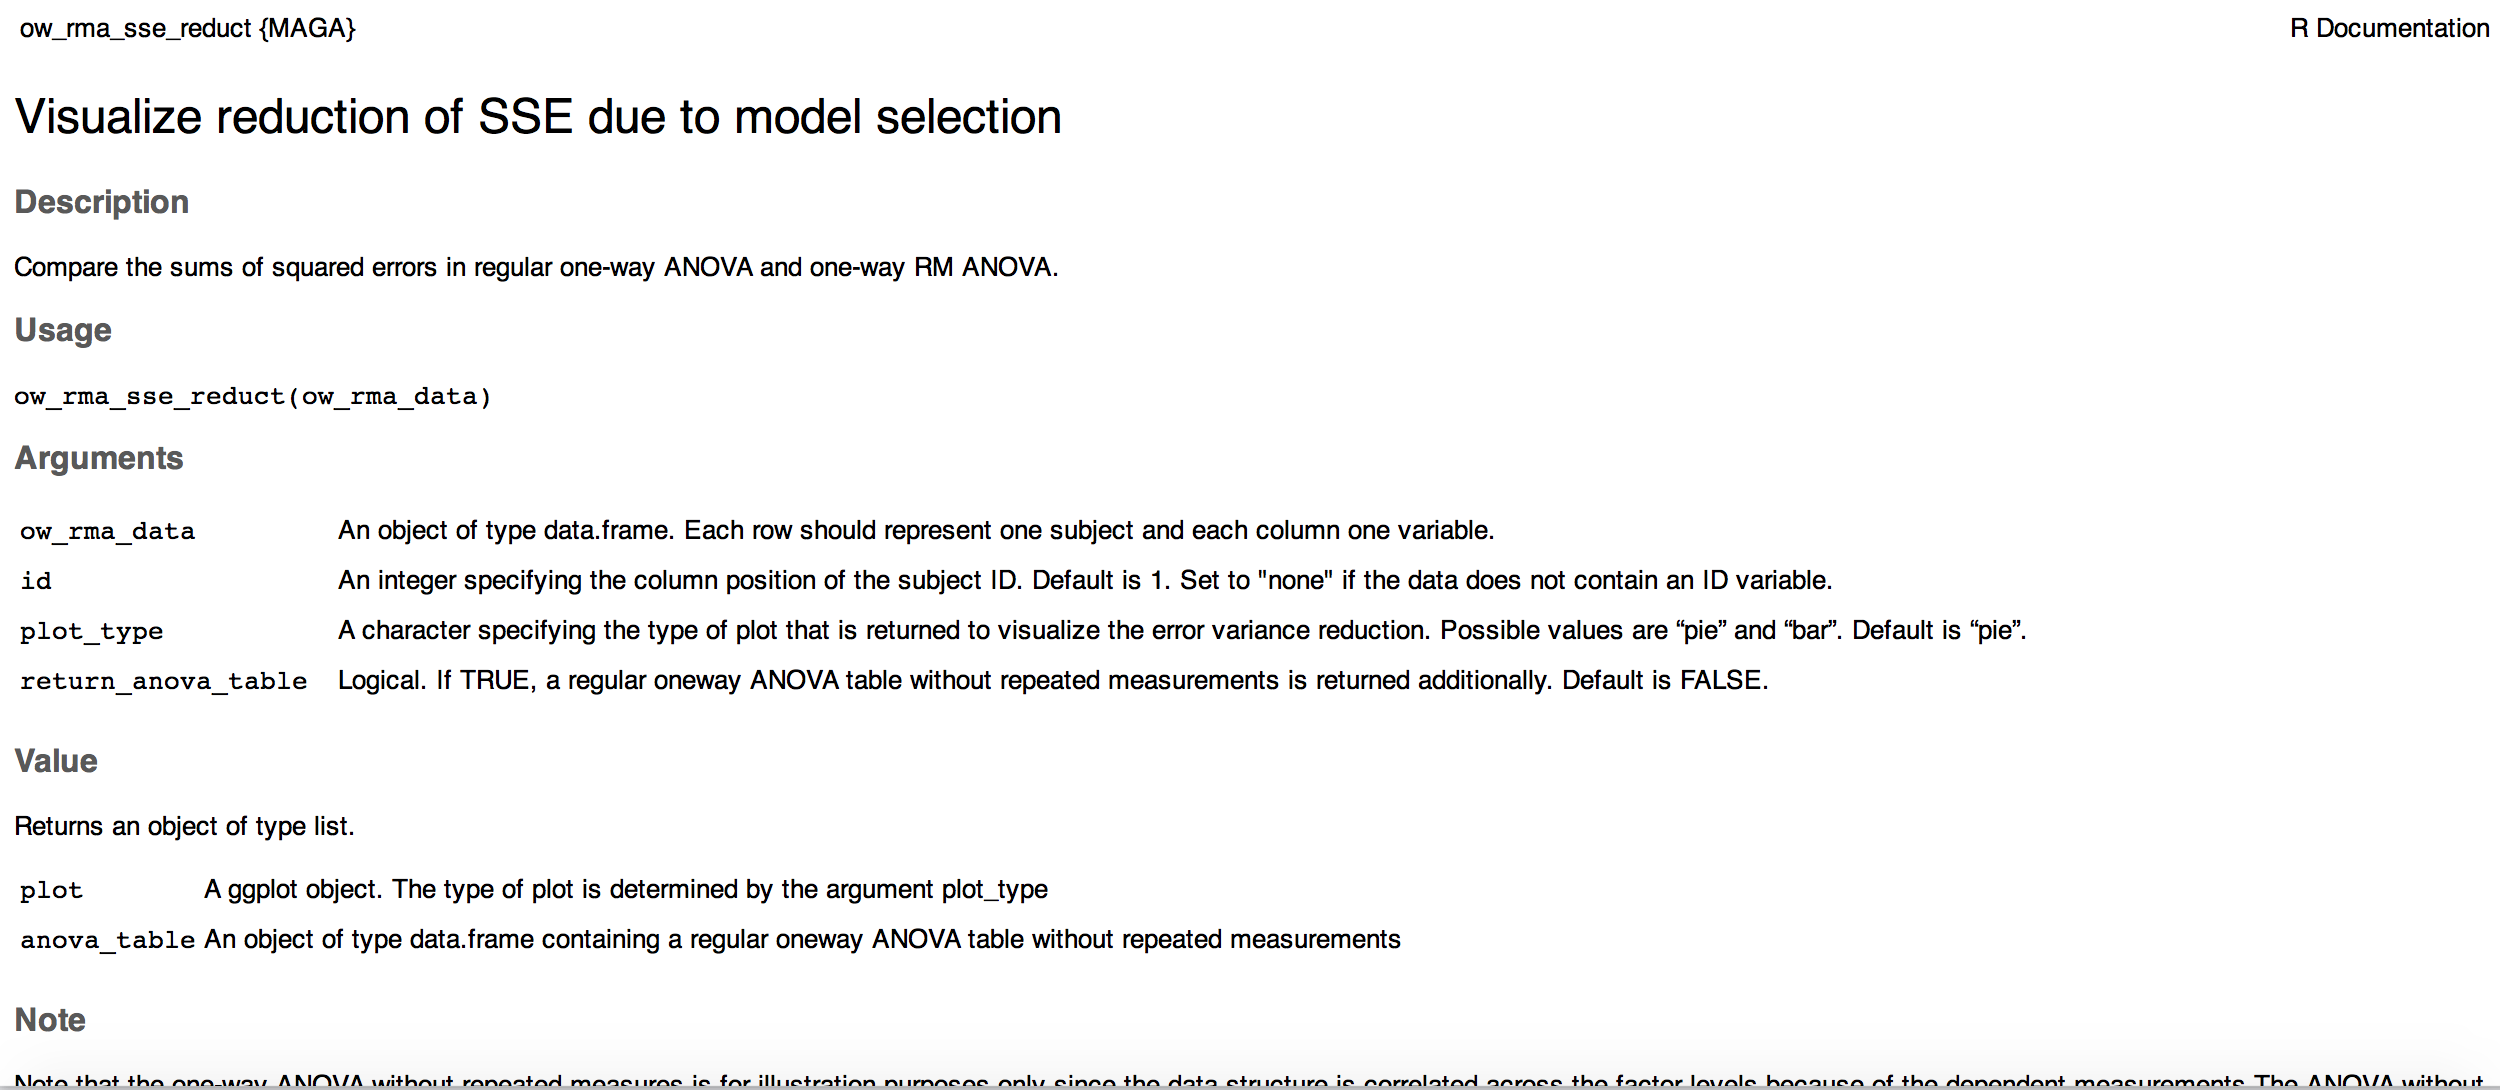
\includegraphics[scale=0.23]{rd_file.png}
		\end{center}
	\end{figure}
}




%%%%%%%%%%%%%%%%%%%%%%%%%%%%%%%%%%%%%%%%%%%%%%%%%%%%%%%%%%%%%%%%%%%%%%%%%%%%%%%%%%%%%%%%%%%%%%%%%%%%%%%%%%%%%%%%%%%%%%%%

\frame[containsverbatim]{
	\frametitle{Package: Things to consider}
	\begin{itemize}
		\item Use function names that speak for themselves and use them consistently.
		\begin{itemize}
			\item \grqq{}There are only two hard things in computer science: cache invalidation and naming things.\grqq{} Phil Karlton
		\end{itemize}
		\item Error handling
		\begin{itemize}
			\item Make sure that functions are robust regarding violation of the required input, e.g. character vector supplied although a numeric vector is needed. Use if-statements or try().
		\end{itemize}
		\item Custom error and warning messages
		\begin{itemize}
			\item stop() interrupts the code and returns an error message
			\item warning() executes the code but returns a warning message
		\end{itemize}
	
	\end{itemize}
}
%%%%%%%%%%%%%%%%%%%%%%%%%%%%%%%%%%%%%%%%%%%%%%%%%%%%%%%%%%%%%%%%%%%%%%%%%%%%%%%%%%%%%%%%%%%%%%%%%%%%%%%%%%%%%%%%%%%%%%%%

\frame[containsverbatim]{
	\frametitle{Thank you for your Attention!}
}
%%%%%%%%%%%%%%%%%%%%%%%%%%%%%%%%%%%%%%%%%%%%%%%%%%%%%%%%%%%%%%%%%%%%%%%%%%%%%%%%%%%%%%%%%%%%%%%%%%%%%%%%%%%%%%%%%%%%%%%%


\frame[containsverbatim]{
	\frametitle{Literature}
	\tiny
	\begin{itemize}
		\item Bakeman, R. (2005). Recommended effect size statistics for repeated measures designs. Behavior Research Methods, 37, 379-384.
		
		\item Box, G. E. R. (1954a). Some theorems on quadratic forms applied in the study of analysis of variance problems. I. Effects of inequality of variance in the one-way classification. Annals of Mathematical Statistics, 25, 484-498.
		
		\item Box, G. E. R. (1954b). Some theorems on quadratic forms applied in the study of analysis of variance problems. II. Effects of inequality of variance and of correlation between errors in the two-way classification. Annals of Mathematical Statistics, 25, 484-498.
		
		\item Geisser, S. \& Greenhouse, S. W. (1958). An extension of Box's results on the use of the F distribution in multivariate analysis. Annals of Mathematical Statistics, 29, 885-891.
		
		\item Huynh, H. \& Feldt, L. S. (1976) Estimation of the Box correction for degrees of freedom from sample data in randomized block and split-plot designs. Journal of Educational Statistics, 1, 69-82.
		
		\item O\' Brien, F. \& Cousineau, D. (2014). Representing error bars in within-subject designs in typical software packages. The Quantitative Methods for Psychology, 10, 58-70.
		
		\item Rutherford, A. (2011): ANOVA and ANCOVA: A GLM Approach (2. Aufl.), Hoboken: John Wiley \& Sons.
		
		
	\end{itemize}
}

%%%%%%%%%%%%%%%%%%%%%%%%%%%%%%%%%%%%%%%%%%%%%%%%%%%%%%%%%%%%%%%%%%%%%%%%%%%%%%%%%%%%%%%%%%%%%%%%%%%%%%%%%%%%%%%%%%%%%%%%

% Define the end of the document:
\end{document}
